%%%%%%%%%%%%%%%%%%%%%%%%%%%%%%%%%%%%%%%
\thesisspacing % CHAPTER
% COPY THEM IN ANY NEW CHAPTER
%%%%%%%%%%%%%%%%%%%%%%%%%%%%%%%%%%%%%%%

This section provides an in-depth analysis of the results obtained from developing and evaluating the Convolutional Neural Network (CNN) model for financial market prediction. The discussion is structured to address the challenges encountered during implementation, the strengths and limitations of the proposed solution, and a quantitative analysis of the model's performance based on the experimental findings.

\section{Challenges in Implementation}

The implementation of the CNN model for financial forecasting posed several significant challenges. One of the most difficult tasks was ensuring that the data used for training was both balanced and representative of various market conditions. Initially, the model struggled with an imbalance in the dataset, leading to a bias in signal prediction, predominantly favoring short signals over long ones. This imbalance necessitated a comprehensive data preprocessing phase where the dataset had to be carefully curated to ensure equal representation of all classifier classes (long, short, and hold). The challenge was further compounded by the limited availability of high-quality financial data, which constrained the volume of data available for training. This limitation required careful selection and preparation of the dataset to ensure it was sufficient to train a robust model without introducing bias.

Another substantial challenge was managing overfitting during the model training phase. The initial model configurations, particularly those with more than 500 million parameters, tended to overfit the training data, especially when the dataset contained outliers or was not sufficiently diverse. Overfitting was mitigated by incorporating techniques such as leaky ReLU activation functions and dropout layers, which helped prevent the model from becoming too tightly fitted to the training data. However, some degree of overfitting remained, suggesting that further refinement of the model architecture or additional data preprocessing techniques could be beneficial.

The backtesting phase presented its own set of challenges. Limited documentation and examples for QSTrader required a deep dive into the framework’s source code to adapt it for the specific needs of this project. Setting up a reliable backtesting environment that accurately reflected real-world trading conditions was crucial for validating the model's performance. Despite these challenges, the backtesting framework ultimately provided valuable insights into the model's practical applicability.

\section{Strengths of the Solution}

Despite the challenges, the solution demonstrated several key strengths that contributed to its overall success. A pivotal strength was the strategic decision to expand the dataset beyond the S\&P 500 index to include a more extensive range of randomly selected U.S. stocks. This expansion significantly enhanced the model's ability to learn from a diverse set of market conditions, allowing it to generalize more effectively. The decision to use data from 30 random stocks, after experimenting with smaller datasets, proved to be optimal. The model’s performance plateaued with more than 30 stocks, indicating that this dataset size was sufficient to capture the necessary market dynamics without introducing redundancy.

Another strength was the flexibility provided by the use of a JSON configuration file for model design. This approach allowed for rapid experimentation with different CNN architectures and hyperparameters, facilitating an efficient iterative development process. The ability to easily modify the model architecture—by adding or removing layers such as convolutional or LSTM layers—enabled the exploration of various configurations, ultimately leading to a more robust model. This flexibility was particularly beneficial in identifying a model structure that exceeded a 50\% accuracy threshold, a critical benchmark for moving forward with backtesting.

The model's ability to identify economic outliers, such as the COVID-19 pandemic period and the market instability in 2022, highlights another strength. The model's recognition of these outlier events, despite being trained on data up to 2017, indicates a strong capacity to generalize from historical data to unprecedented market conditions. This capability is crucial for financial forecasting, where the ability to anticipate rare but impactful events can significantly affect portfolio performance.

\section{Limitations of the Solution}

While the solution demonstrated significant strengths, it also had notable limitations that need to be addressed. A primary limitation was the model's initial bias towards generating only long or short signals, a problem rooted in the dataset's imbalance. Although balancing the data resolved this issue to some extent, it also reduced the amount of data available for training, potentially limiting the model's ability to learn from a broader range of scenarios. This trade-off highlights a fundamental challenge in machine learning: balancing the need for diverse, representative training data with the need to maintain sufficient dataset size for robust model training.

The tendency of the model to overfit, particularly when using a highly complex architecture, also presented a significant limitation. While the introduction of dropout layers and leaky ReLU activations helped mitigate this issue, the model still exhibited signs of overfitting, particularly when exposed to outlier data points. This suggests that further refinement is needed, either through more advanced regularization techniques or by improving the quality and diversity of the training data.

Another limitation was the model's initial approach to handling multiple asset classes, including equities, currencies, and bonds. This approach proved to be overly ambitious, given the model's architecture and the data limitations. The model was unable to effectively capture the diverse information needed to make accurate predictions across multiple asset classes, resulting in suboptimal performance. Simplifying the model to focus solely on randomly selected U.S. stocks led to better results, but this approach also reduced the model's applicability to broader market contexts.


\section{Quantitative Findings}

The quantitative findings of this study provide a clear comparison between the well-performing and poorly performing models. The well-trained model, optimized using data from 30 randomly selected U.S. stocks, achieved a Sharpe ratio of 1.20 and maintained a drawdown of 24.46\%. These metrics indicate a significantly better risk-adjusted return compared to the poorly performing model, which recorded a Sharpe ratio of 0.19 and a drawdown of 49.63\%. The well-performing model also exhibited a positive Compound Annual Growth Rate (CAGR) of 24.74\%, in contrast to the negative CAGR of -5.50\% for the poorly performing model, underscoring its effectiveness in leveraging market opportunities while minimizing potential losses.

Despite the similar levels of volatility between the two models, the marked difference in their CAGRs and drawdowns underscores the importance of effective model training and careful data selection in building robust financial forecasting tools. The well-trained model's capacity to perform effectively during periods of market instability, such as the COVID-19 pandemic, further highlights its robustness and adaptability to varying market conditions.

Additionally, the analysis of trade distribution and mean returns provides further insight into the model's trading strategy. As shown in Figure~\ref{fig:trade_distribution}, the distribution of trades with their corresponding mean returns and standard deviations indicates a positive mean return across most months, suggesting that the model was generally effective in identifying profitable trading opportunities. This consistency in generating positive returns, even with a degree of variability, demonstrates the model’s potential reliability in real-world trading scenarios.

Overall, the quantitative results highlight both the strengths and limitations of the proposed CNN model for financial forecasting. The well-trained model's ability to maintain a positive risk-adjusted performance and its capacity to adapt to unstable market periods provide a strong foundation for further refinement and development.

\begin{figure}[h!]
    \centering
    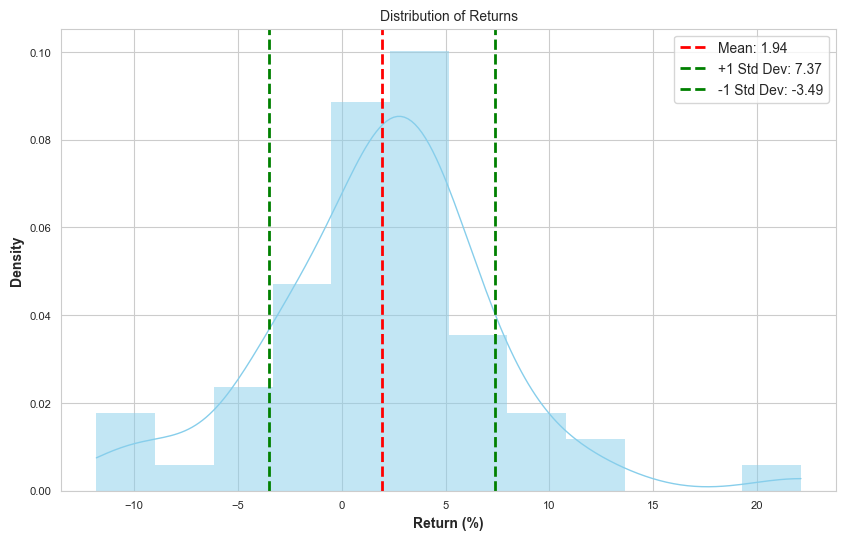
\includegraphics[width=0.7\textwidth]{chapters/Chap4/Monthly_Distribution.png}
    \caption{Distribution of trades with mean returns and standard deviations, showing a generally positive mean return across most months.}
    \label{fig:trade_distribution}
\end{figure}
